\begin{figure}[ht]
    \tikzstyle{startstop} = [rectangle, minimum width = 1.5cm, minimum height = 0.5cm, text centered, draw = black]
    \tikzstyle{arrow} = [thick, ->]
    
    \centering
    
    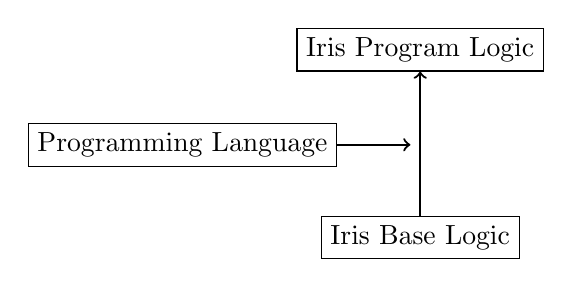
\begin{tikzpicture}[node distance = 1.5cm]

    \node(base)[startstop] {Iris Base Logic};
    \node(mid)[above=30] at (base) {};
    \node(lang)[startstop, left=30] at (mid) {Programming Language};
    \node(logic)[startstop, above=60] at (base) {Iris Program Logic};

    \draw[arrow](base) -- (logic);
    \draw[arrow](lang) -- (mid);
    
    \end{tikzpicture}
    \caption{Iris Framework}
    \label{fig:iris-framework}
\end{figure}